Permite seleccionar el día y la hora de inicio y la duración en la que será reservada la sala.

\subsection{Subpaso 3-A: Seleccionar día de la reservación}
\begin{enumerate}
	\item Seleccione el mes en el que se va a hacer el préstamo 
		\textbf{IUGS-03 día}.
	\item Presione el día en el que se va a hacer el préstamo.
	\item De clic en uno de los bloques de tiempo libre de sala que 
		desea reservar.
	\item Ingrese la hora de inicio de la reservación.
	\item Ingrese la hora de finalización de la reservación.
	\item Presione el botón de \textbf{Aceptar}.
\end{enumerate}

\textbf{Restricción 1.} Una sala debe reservarse con, al menos, tres
	días de antelación y máximo tres semanas antes.
	\begin{figure}
	
\includegraphics[scale=0.3]{images/InterfazMovil/IUGS02_reservarDiaSolicitante.png}
		\caption{Reservar fecha solicitante}
	\end{figure}
	
	
		\begin{figure}
	
\includegraphics[scale=0.3]{images/InterfazMovil/IUGS02_reservarHoraSolicitante.png}
		\caption{Reservar fecha solicitante}
	\end{figure}
	
	\begin{figure}
	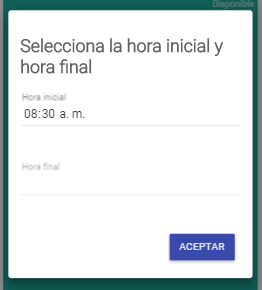
\includegraphics[scale=0.3]{images/InterfazMovil/IUGS02_reservarHoraEstableSolicitante.png}
		\caption{Reservar fecha solicitante}
	\end{figure}
	